% Options for packages loaded elsewhere
\PassOptionsToPackage{unicode}{hyperref}
\PassOptionsToPackage{hyphens}{url}
\PassOptionsToPackage{dvipsnames,svgnames,x11names}{xcolor}
%
\documentclass[
  letterpaper,
  DIV=11,
  numbers=noendperiod]{scrreprt}

\usepackage{amsmath,amssymb}
\usepackage{iftex}
\ifPDFTeX
  \usepackage[T1]{fontenc}
  \usepackage[utf8]{inputenc}
  \usepackage{textcomp} % provide euro and other symbols
\else % if luatex or xetex
  \usepackage{unicode-math}
  \defaultfontfeatures{Scale=MatchLowercase}
  \defaultfontfeatures[\rmfamily]{Ligatures=TeX,Scale=1}
\fi
\usepackage{lmodern}
\ifPDFTeX\else  
    % xetex/luatex font selection
\fi
% Use upquote if available, for straight quotes in verbatim environments
\IfFileExists{upquote.sty}{\usepackage{upquote}}{}
\IfFileExists{microtype.sty}{% use microtype if available
  \usepackage[]{microtype}
  \UseMicrotypeSet[protrusion]{basicmath} % disable protrusion for tt fonts
}{}
\makeatletter
\@ifundefined{KOMAClassName}{% if non-KOMA class
  \IfFileExists{parskip.sty}{%
    \usepackage{parskip}
  }{% else
    \setlength{\parindent}{0pt}
    \setlength{\parskip}{6pt plus 2pt minus 1pt}}
}{% if KOMA class
  \KOMAoptions{parskip=half}}
\makeatother
\usepackage{xcolor}
\setlength{\emergencystretch}{3em} % prevent overfull lines
\setcounter{secnumdepth}{5}
% Make \paragraph and \subparagraph free-standing
\makeatletter
\ifx\paragraph\undefined\else
  \let\oldparagraph\paragraph
  \renewcommand{\paragraph}{
    \@ifstar
      \xxxParagraphStar
      \xxxParagraphNoStar
  }
  \newcommand{\xxxParagraphStar}[1]{\oldparagraph*{#1}\mbox{}}
  \newcommand{\xxxParagraphNoStar}[1]{\oldparagraph{#1}\mbox{}}
\fi
\ifx\subparagraph\undefined\else
  \let\oldsubparagraph\subparagraph
  \renewcommand{\subparagraph}{
    \@ifstar
      \xxxSubParagraphStar
      \xxxSubParagraphNoStar
  }
  \newcommand{\xxxSubParagraphStar}[1]{\oldsubparagraph*{#1}\mbox{}}
  \newcommand{\xxxSubParagraphNoStar}[1]{\oldsubparagraph{#1}\mbox{}}
\fi
\makeatother

\usepackage{color}
\usepackage{fancyvrb}
\newcommand{\VerbBar}{|}
\newcommand{\VERB}{\Verb[commandchars=\\\{\}]}
\DefineVerbatimEnvironment{Highlighting}{Verbatim}{commandchars=\\\{\}}
% Add ',fontsize=\small' for more characters per line
\usepackage{framed}
\definecolor{shadecolor}{RGB}{241,243,245}
\newenvironment{Shaded}{\begin{snugshade}}{\end{snugshade}}
\newcommand{\AlertTok}[1]{\textcolor[rgb]{0.68,0.00,0.00}{#1}}
\newcommand{\AnnotationTok}[1]{\textcolor[rgb]{0.37,0.37,0.37}{#1}}
\newcommand{\AttributeTok}[1]{\textcolor[rgb]{0.40,0.45,0.13}{#1}}
\newcommand{\BaseNTok}[1]{\textcolor[rgb]{0.68,0.00,0.00}{#1}}
\newcommand{\BuiltInTok}[1]{\textcolor[rgb]{0.00,0.23,0.31}{#1}}
\newcommand{\CharTok}[1]{\textcolor[rgb]{0.13,0.47,0.30}{#1}}
\newcommand{\CommentTok}[1]{\textcolor[rgb]{0.37,0.37,0.37}{#1}}
\newcommand{\CommentVarTok}[1]{\textcolor[rgb]{0.37,0.37,0.37}{\textit{#1}}}
\newcommand{\ConstantTok}[1]{\textcolor[rgb]{0.56,0.35,0.01}{#1}}
\newcommand{\ControlFlowTok}[1]{\textcolor[rgb]{0.00,0.23,0.31}{\textbf{#1}}}
\newcommand{\DataTypeTok}[1]{\textcolor[rgb]{0.68,0.00,0.00}{#1}}
\newcommand{\DecValTok}[1]{\textcolor[rgb]{0.68,0.00,0.00}{#1}}
\newcommand{\DocumentationTok}[1]{\textcolor[rgb]{0.37,0.37,0.37}{\textit{#1}}}
\newcommand{\ErrorTok}[1]{\textcolor[rgb]{0.68,0.00,0.00}{#1}}
\newcommand{\ExtensionTok}[1]{\textcolor[rgb]{0.00,0.23,0.31}{#1}}
\newcommand{\FloatTok}[1]{\textcolor[rgb]{0.68,0.00,0.00}{#1}}
\newcommand{\FunctionTok}[1]{\textcolor[rgb]{0.28,0.35,0.67}{#1}}
\newcommand{\ImportTok}[1]{\textcolor[rgb]{0.00,0.46,0.62}{#1}}
\newcommand{\InformationTok}[1]{\textcolor[rgb]{0.37,0.37,0.37}{#1}}
\newcommand{\KeywordTok}[1]{\textcolor[rgb]{0.00,0.23,0.31}{\textbf{#1}}}
\newcommand{\NormalTok}[1]{\textcolor[rgb]{0.00,0.23,0.31}{#1}}
\newcommand{\OperatorTok}[1]{\textcolor[rgb]{0.37,0.37,0.37}{#1}}
\newcommand{\OtherTok}[1]{\textcolor[rgb]{0.00,0.23,0.31}{#1}}
\newcommand{\PreprocessorTok}[1]{\textcolor[rgb]{0.68,0.00,0.00}{#1}}
\newcommand{\RegionMarkerTok}[1]{\textcolor[rgb]{0.00,0.23,0.31}{#1}}
\newcommand{\SpecialCharTok}[1]{\textcolor[rgb]{0.37,0.37,0.37}{#1}}
\newcommand{\SpecialStringTok}[1]{\textcolor[rgb]{0.13,0.47,0.30}{#1}}
\newcommand{\StringTok}[1]{\textcolor[rgb]{0.13,0.47,0.30}{#1}}
\newcommand{\VariableTok}[1]{\textcolor[rgb]{0.07,0.07,0.07}{#1}}
\newcommand{\VerbatimStringTok}[1]{\textcolor[rgb]{0.13,0.47,0.30}{#1}}
\newcommand{\WarningTok}[1]{\textcolor[rgb]{0.37,0.37,0.37}{\textit{#1}}}

\providecommand{\tightlist}{%
  \setlength{\itemsep}{0pt}\setlength{\parskip}{0pt}}\usepackage{longtable,booktabs,array}
\usepackage{calc} % for calculating minipage widths
% Correct order of tables after \paragraph or \subparagraph
\usepackage{etoolbox}
\makeatletter
\patchcmd\longtable{\par}{\if@noskipsec\mbox{}\fi\par}{}{}
\makeatother
% Allow footnotes in longtable head/foot
\IfFileExists{footnotehyper.sty}{\usepackage{footnotehyper}}{\usepackage{footnote}}
\makesavenoteenv{longtable}
\usepackage{graphicx}
\makeatletter
\newsavebox\pandoc@box
\newcommand*\pandocbounded[1]{% scales image to fit in text height/width
  \sbox\pandoc@box{#1}%
  \Gscale@div\@tempa{\textheight}{\dimexpr\ht\pandoc@box+\dp\pandoc@box\relax}%
  \Gscale@div\@tempb{\linewidth}{\wd\pandoc@box}%
  \ifdim\@tempb\p@<\@tempa\p@\let\@tempa\@tempb\fi% select the smaller of both
  \ifdim\@tempa\p@<\p@\scalebox{\@tempa}{\usebox\pandoc@box}%
  \else\usebox{\pandoc@box}%
  \fi%
}
% Set default figure placement to htbp
\def\fps@figure{htbp}
\makeatother

\KOMAoption{captions}{tableheading}
\makeatletter
\@ifpackageloaded{bookmark}{}{\usepackage{bookmark}}
\makeatother
\makeatletter
\@ifpackageloaded{caption}{}{\usepackage{caption}}
\AtBeginDocument{%
\ifdefined\contentsname
  \renewcommand*\contentsname{Table of contents}
\else
  \newcommand\contentsname{Table of contents}
\fi
\ifdefined\listfigurename
  \renewcommand*\listfigurename{List of Figures}
\else
  \newcommand\listfigurename{List of Figures}
\fi
\ifdefined\listtablename
  \renewcommand*\listtablename{List of Tables}
\else
  \newcommand\listtablename{List of Tables}
\fi
\ifdefined\figurename
  \renewcommand*\figurename{Figure}
\else
  \newcommand\figurename{Figure}
\fi
\ifdefined\tablename
  \renewcommand*\tablename{Table}
\else
  \newcommand\tablename{Table}
\fi
}
\@ifpackageloaded{float}{}{\usepackage{float}}
\floatstyle{ruled}
\@ifundefined{c@chapter}{\newfloat{codelisting}{h}{lop}}{\newfloat{codelisting}{h}{lop}[chapter]}
\floatname{codelisting}{Listing}
\newcommand*\listoflistings{\listof{codelisting}{List of Listings}}
\makeatother
\makeatletter
\makeatother
\makeatletter
\@ifpackageloaded{caption}{}{\usepackage{caption}}
\@ifpackageloaded{subcaption}{}{\usepackage{subcaption}}
\makeatother

\usepackage{bookmark}

\IfFileExists{xurl.sty}{\usepackage{xurl}}{} % add URL line breaks if available
\urlstyle{same} % disable monospaced font for URLs
\hypersetup{
  pdftitle={Secondary Malaria Data Sources},
  pdfauthor={Amir Siraj},
  colorlinks=true,
  linkcolor={blue},
  filecolor={Maroon},
  citecolor={Blue},
  urlcolor={Blue},
  pdfcreator={LaTeX via pandoc}}


\title{Secondary Malaria Data Sources}
\author{Amir Siraj}
\date{2024-10-30}

\begin{document}
\maketitle

\renewcommand*\contentsname{Table of contents}
{
\hypersetup{linkcolor=}
\setcounter{tocdepth}{2}
\tableofcontents
}

\bookmarksetup{startatroot}

\chapter*{Preface}\label{preface}
\addcontentsline{toc}{chapter}{Preface}

\markboth{Preface}{Preface}

Vector control constitutes a major component of malaria control and
elimination strategies. WHO recommends using insecticide-treated nets
(ITNs) and/ or indoor residual spraying (IRS) for malaria vector control
in most areas at risk of malaria as appropriate. These interventions may
be supplemented by other interventions such as larval source management
(LSM) depending on the setting and available resources.

In the first module, we will discuss the main vector control
interventions, i.e., LLIN and IRS, in more detail. The second module
deals with data from the Demographic and Health Survey (DHS) program.

\bookmarksetup{startatroot}

\chapter{Insecticide treated nets}\label{insecticide-treated-nets}

MACEPA Data Fellowship - Training Materials

\hfill\break

Insecticide-treated bed nets (ITNs) are a form of personal protection
that can reduce the risk of malaria illness, severe disease, and death.
In community-wide trials in several African settings, ITNs reduced the
death of children under 5 years from all causes by about 20\%. ITNs
repel, kill, or sterilize mosquitoes that come into contact with the
insecticides or other active ingredients impregnated on the netting
material. ITNs also have a community effect where members of the
community (not just those who sleep under a net) may have some
protection when a large proportion of the community uses ITNs.~The
effectiveness of ITNs diminishes over time due to physical damage,
deteriorating chemical integrity, or bio-efficacy (i.e., through the
development of insecticide resistance).~ Long-lasting insecticidal net
(LLIN) is a special type of ITN that stays effective for a longer time
(\textasciitilde{} 3 years) before replacement, without a need for
reimpregnation with insecticide.~

\bookmarksetup{startatroot}

\chapter{\texorpdfstring{\textbf{ITN distribution
data}}{ITN distribution data}}\label{itn-distribution-data}

For seceral decades, ITNs and LLINs have been delivered to
malaria-endemic countries through various global or local initiatives
and programs. National Malaria Control Programs (NMCPs) in endemic
countries coordinate the distribution of bed nets to target
populations.~ In most countries, ITN distributions are mainly carried
out in two formats:

\begin{itemize}
\item
  \textbf{Mass ITN campaign}: is a cost-effective way of rapidly
  achieving high and equitable vector control coverages. ITN campaigns
  are done once every few years targeting all or a cohort of population
  at each round (usually districts but can be at lower administrative
  units too), They aim to provide a proportion of the population in the
  target districts with new ITNs at a regular interval (ideally every 3
  years).
\item
  \textbf{Routine programs}: Routine antenatal and immunization services
  program provides a cost-effective means to reach out to communities at
  a higher risk of malaria transmission including children and mothers.
  Programs keep stocks of ITNs which they dispense to beneficiaries
  along with their routine services.

  Most NMEPs compile data on the number of ITNs distributed at the
  district level or sub-district levels on annual basis. In recent
  years, ITN distribution data have been incorporated into the DHIS-2
  system improving their accessibility. Access to this data (usually
  through the NMEPs) ensures data is used in analytics and modeling
  related works.
\end{itemize}

\section{Working with LLIN data from
NMEP}\label{working-with-llin-data-from-nmep}

\subsection{\texorpdfstring{\textbf{Mass LLIN distribution
data}}{Mass LLIN distribution data}}\label{mass-llin-distribution-data}

In this exercise, we will look at an example of mock data for sample
districts in Ethiopia. Note that the data we use in this exercise is
made up and may not have any use outside this exercise. This exercise
assumes the LLIN data and accompanying population figures have been
cleaned and verified for consistency and completeness.

First, let us load the necessary libraries.~~~

\begin{Shaded}
\begin{Highlighting}[]
\FunctionTok{library}\NormalTok{(tidyverse)}
\end{Highlighting}
\end{Shaded}

\begin{verbatim}
-- Attaching core tidyverse packages ------------------------ tidyverse 2.0.0 --
v dplyr     1.1.4     v readr     2.1.5
v forcats   1.0.0     v stringr   1.5.1
v ggplot2   3.5.2     v tibble    3.3.0
v lubridate 1.9.4     v tidyr     1.3.1
v purrr     1.1.0     
-- Conflicts ------------------------------------------ tidyverse_conflicts() --
x dplyr::filter() masks stats::filter()
x dplyr::lag()    masks stats::lag()
i Use the conflicted package (<http://conflicted.r-lib.org/>) to force all conflicts to become errors
\end{verbatim}

\begin{Shaded}
\begin{Highlighting}[]
\FunctionTok{library}\NormalTok{(lubridate)}
\end{Highlighting}
\end{Shaded}

We will read data on mass campaign LLIN distribution obtained from NMEP
to support our analysis. We will further read the~corresponding
population data for each district.

\begin{Shaded}
\begin{Highlighting}[]
\NormalTok{mass\_llin\_dist}\OtherTok{\textless{}{-}} \FunctionTok{read\_csv}\NormalTok{(}\StringTok{"data/llin\_mass\_2017\_2020.csv"}\NormalTok{) }
\end{Highlighting}
\end{Shaded}

\begin{verbatim}
Rows: 300 Columns: 7
-- Column specification --------------------------------------------------------
Delimiter: ","
chr (3): region, zone, district
dbl (4): llin_2017, llin_2018, llin_2019, llin_2020

i Use `spec()` to retrieve the full column specification for this data.
i Specify the column types or set `show_col_types = FALSE` to quiet this message.
\end{verbatim}

\begin{Shaded}
\begin{Highlighting}[]
\NormalTok{population}\OtherTok{\textless{}{-}} \FunctionTok{read\_csv}\NormalTok{(}\StringTok{"data/pop\_2017\_2020.csv"}\NormalTok{)}
\end{Highlighting}
\end{Shaded}

\begin{verbatim}
Rows: 300 Columns: 7
-- Column specification --------------------------------------------------------
Delimiter: ","
chr (3): region, zone, district
dbl (4): pop_2017, pop_2018, pop_2019, pop_2020

i Use `spec()` to retrieve the full column specification for this data.
i Specify the column types or set `show_col_types = FALSE` to quiet this message.
\end{verbatim}

We can visualize and verify if our data is consistent with the
expectation. To do that we join the LLIN distribution datasets with the
corresponding population data.

The following script does that by (a) converting the datasets into long
format (b) joining them based on geographic units and years, and (c)
generating LLINs per population (as an indicator of access to LLIN).

\begin{Shaded}
\begin{Highlighting}[]
\DocumentationTok{\#\#\# convert mass LLIN data into long format}
\NormalTok{mass\_llin\_long}\OtherTok{\textless{}{-}} 
\NormalTok{  mass\_llin\_dist }\SpecialCharTok{|\textgreater{}}
  \FunctionTok{pivot\_longer}\NormalTok{(}\AttributeTok{cols =} \FunctionTok{contains}\NormalTok{(}\StringTok{"llin"}\NormalTok{),}
               \AttributeTok{names\_to =} \StringTok{"year\_txt"}\NormalTok{, }
               \AttributeTok{values\_to =} \StringTok{"llin"}\NormalTok{) }\SpecialCharTok{|\textgreater{}}
  \FunctionTok{mutate}\NormalTok{(}\AttributeTok{year =} \FunctionTok{as.numeric}\NormalTok{(}\FunctionTok{substr}\NormalTok{(year\_txt,}\DecValTok{6}\NormalTok{,}\DecValTok{9}\NormalTok{))) }\SpecialCharTok{|\textgreater{}}
\NormalTok{  dplyr}\SpecialCharTok{::}\FunctionTok{select}\NormalTok{(}\SpecialCharTok{{-}}\NormalTok{year\_txt)}

\DocumentationTok{\#\#\# convert population data into long format}
\NormalTok{population\_long}\OtherTok{\textless{}{-}}\NormalTok{ population }\SpecialCharTok{|\textgreater{}}
  \FunctionTok{pivot\_longer}\NormalTok{(}\AttributeTok{cols =} \FunctionTok{contains}\NormalTok{(}\StringTok{"pop"}\NormalTok{),}
               \AttributeTok{names\_to =} \StringTok{"year\_txt"}\NormalTok{,}
               \AttributeTok{values\_to =} \StringTok{"pop"}\NormalTok{)}\SpecialCharTok{|\textgreater{}}
  \FunctionTok{mutate}\NormalTok{(}\AttributeTok{year =} \FunctionTok{as.numeric}\NormalTok{(}\FunctionTok{substr}\NormalTok{(year\_txt,}\DecValTok{5}\NormalTok{,}\DecValTok{8}\NormalTok{))) }\SpecialCharTok{|\textgreater{}}
\NormalTok{  dplyr}\SpecialCharTok{::}\FunctionTok{select}\NormalTok{(}\SpecialCharTok{{-}}\NormalTok{year\_txt)}

\DocumentationTok{\#\#\# join the two and generate llin per person}
\NormalTok{  mllin\_pop }\OtherTok{=}\NormalTok{ mass\_llin\_long }\SpecialCharTok{|\textgreater{}}
  \FunctionTok{left\_join}\NormalTok{(population\_long,}
            \AttributeTok{by =} \FunctionTok{c}\NormalTok{(}\StringTok{"region"}\NormalTok{,}
                   \StringTok{"zone"}\NormalTok{,}
                   \StringTok{"district"}\NormalTok{,}
                   \StringTok{"year"}\NormalTok{)) }\SpecialCharTok{|\textgreater{}}
    \FunctionTok{mutate}\NormalTok{(}\AttributeTok{llin\_per\_person  =}\NormalTok{ llin}\SpecialCharTok{/}\NormalTok{pop)}


\DocumentationTok{\#\#\# visualize}
\NormalTok{mllin\_pop}\SpecialCharTok{|\textgreater{}} 
    \FunctionTok{filter}\NormalTok{(llin\_per\_person}\SpecialCharTok{\textgreater{}}\DecValTok{0}\NormalTok{) }\SpecialCharTok{|\textgreater{}}
    \FunctionTok{ggplot}\NormalTok{(}\FunctionTok{aes}\NormalTok{(}\AttributeTok{x=}\NormalTok{year, }\AttributeTok{y =}\NormalTok{ llin\_per\_person)) }\SpecialCharTok{+}
    \FunctionTok{facet\_wrap}\NormalTok{ (}\SpecialCharTok{\textasciitilde{}}\NormalTok{ district) }\SpecialCharTok{+}
    \FunctionTok{geom\_point}\NormalTok{()}
\end{Highlighting}
\end{Shaded}

\pandocbounded{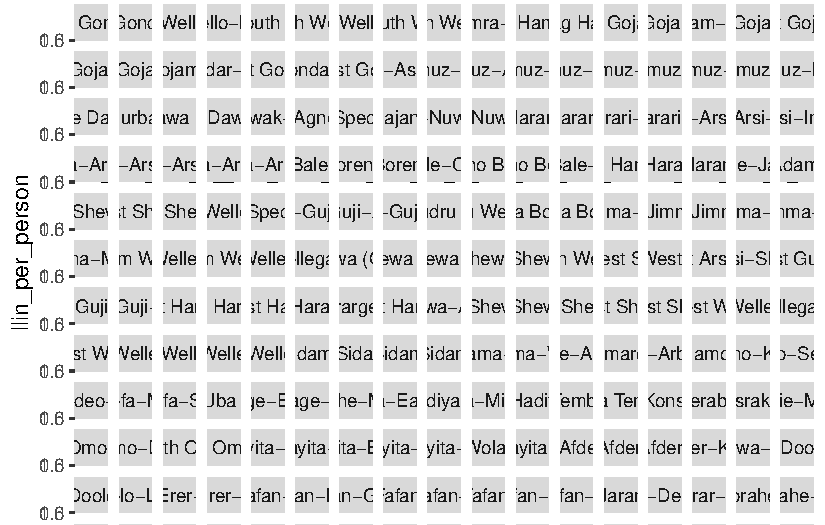
\includegraphics[keepaspectratio]{module_01_files/figure-pdf/unnamed-chunk-3-1.pdf}}

\begin{Shaded}
\begin{Highlighting}[]
  \FunctionTok{ggsave}\NormalTok{(}\AttributeTok{filename =} \StringTok{"plots/llin\_mass.tiff"}\NormalTok{,}
         \AttributeTok{width =} \DecValTok{8}\NormalTok{, }\AttributeTok{height =} \DecValTok{10}\NormalTok{, }\AttributeTok{compression =} \StringTok{"lzw"}\NormalTok{)}
\end{Highlighting}
\end{Shaded}

Mass distributions often assume two persons would use a single LLIN. In
other words, 100\% coverage would be achieved if a district gets LLIN
about half its population. Thus, it would be somewhat curious if a
district reports LLIN per person greater than 0.5, and even more
suspicious if they report figures greater than 1. Note that the data
quality issues can come from one or both of the two data sets used, mass
LLIN~ and the population denominator.

\pandocbounded{
\includegraphics[keepaspectratio]{plots/image_01.png}}\hfill

\textbf{Exercise 1:} How many districts in the above example reported
LLIN per person values greater than 1 in any year?

\subsection{\texorpdfstring{\textbf{Routine LLIN distribution
data}}{Routine LLIN distribution data}}\label{routine-llin-distribution-data}

In this exercise, we will look at an example of mock routine LLIN
distribution data for the sample districts. This exercise assumes the
LLIN data and accompanying population figures have been cleaned and
verified for consistency and completeness.

First, let us load the necessary libraries.~~~

\begin{Shaded}
\begin{Highlighting}[]
\FunctionTok{library}\NormalTok{(tidyverse)}
\FunctionTok{library}\NormalTok{(lubridate)}
\end{Highlighting}
\end{Shaded}

We will read data on LLIN distribution through routine programs (EPI and
ANC). We will further read the~corresponding population data for each
district.

\begin{Shaded}
\begin{Highlighting}[]
\NormalTok{routine\_llin\_dist}\OtherTok{\textless{}{-}} \FunctionTok{read\_csv}\NormalTok{(}\StringTok{"data/llin\_routine\_2017\_2020.csv"}\NormalTok{) }
\end{Highlighting}
\end{Shaded}

\begin{verbatim}
Rows: 1200 Columns: 12
-- Column specification --------------------------------------------------------
Delimiter: ","
chr (3): region, zone, district
dbl (9): year, llins_epi_u6m, llins_epi_611m, llins_epi_1223m, llins_epi_245...

i Use `spec()` to retrieve the full column specification for this data.
i Specify the column types or set `show_col_types = FALSE` to quiet this message.
\end{verbatim}

\begin{Shaded}
\begin{Highlighting}[]
\NormalTok{population}\OtherTok{\textless{}{-}} \FunctionTok{read\_csv}\NormalTok{(}\StringTok{"data/pop\_2017\_2020.csv"}\NormalTok{)}
\end{Highlighting}
\end{Shaded}

\begin{verbatim}
Rows: 300 Columns: 7
-- Column specification --------------------------------------------------------
Delimiter: ","
chr (3): region, zone, district
dbl (4): pop_2017, pop_2018, pop_2019, pop_2020

i Use `spec()` to retrieve the full column specification for this data.
i Specify the column types or set `show_col_types = FALSE` to quiet this message.
\end{verbatim}

We can visualize and verify if our data is consistent with the
expectation. To do that we join the LLIN distribution datasets with the
corresponding population data.

The following script does that by (a) converting the datasets into long
format (b) joining them based on geographic units and years, and (c)
generating LLINs per estimated population under five years old by
assuming U5 population is roughly a fifth of the overall population.

\begin{Shaded}
\begin{Highlighting}[]
\DocumentationTok{\#\#\# convert routine LLIN data into long format}
\NormalTok{routine\_llin\_long}\OtherTok{\textless{}{-}}\NormalTok{ routine\_llin\_dist }\SpecialCharTok{|\textgreater{}}
  \FunctionTok{pivot\_longer}\NormalTok{(}\AttributeTok{cols =} \FunctionTok{contains}\NormalTok{(}\StringTok{"llin"}\NormalTok{),}
               \AttributeTok{names\_to =} \StringTok{"program"}\NormalTok{,}
               \AttributeTok{values\_to =} \StringTok{"llin"}\NormalTok{)}

\DocumentationTok{\#\#\# convert population data into long format}
\NormalTok{population\_long}\OtherTok{\textless{}{-}}\NormalTok{ population }\SpecialCharTok{|\textgreater{}}
  \FunctionTok{pivot\_longer}\NormalTok{(}\AttributeTok{cols =} \FunctionTok{contains}\NormalTok{(}\StringTok{"pop"}\NormalTok{),}
               \AttributeTok{names\_to =} \StringTok{"year\_txt"}\NormalTok{, }
               \AttributeTok{values\_to =} \StringTok{"pop"}\NormalTok{) }\SpecialCharTok{|\textgreater{}}
  \FunctionTok{mutate}\NormalTok{(}\AttributeTok{year =} \FunctionTok{as.numeric}\NormalTok{(}\FunctionTok{substr}\NormalTok{(year\_txt,}\DecValTok{5}\NormalTok{,}\DecValTok{8}\NormalTok{))) }\SpecialCharTok{|\textgreater{}}
\NormalTok{  dplyr}\SpecialCharTok{::}\FunctionTok{select}\NormalTok{(}\SpecialCharTok{{-}}\NormalTok{year\_txt)}


\DocumentationTok{\#\#\# join the two and generate llin per person}

\NormalTok{rllin\_pop }\OtherTok{\textless{}{-}}\NormalTok{   routine\_llin\_long }\SpecialCharTok{|\textgreater{}}
  \FunctionTok{left\_join}\NormalTok{(population\_long,}
            \AttributeTok{by =} \FunctionTok{c}\NormalTok{(}\StringTok{"region"}\NormalTok{,}
                   \StringTok{"zone"}\NormalTok{,}
                   \StringTok{"district"}\NormalTok{,}
                   \StringTok{"year"}\NormalTok{)) }\SpecialCharTok{|\textgreater{}}
  \FunctionTok{group\_by}\NormalTok{(region, zone, district, year) }\SpecialCharTok{|\textgreater{}}
  \FunctionTok{summarise}\NormalTok{(}\AttributeTok{rllin =} \FunctionTok{sum}\NormalTok{(llin, }\AttributeTok{na.rm=}\NormalTok{T),}
            \AttributeTok{population =} \FunctionTok{mean}\NormalTok{(pop)) }\SpecialCharTok{|\textgreater{}}
  \FunctionTok{ungroup}\NormalTok{() }\SpecialCharTok{|\textgreater{}}
  \FunctionTok{mutate}\NormalTok{(}\AttributeTok{llin\_per\_u5  =}\NormalTok{ rllin}\SpecialCharTok{/}\NormalTok{population }\SpecialCharTok{*} \DecValTok{5}\NormalTok{)  }\CommentTok{\# assuming U5 a fifth of pop.}
\end{Highlighting}
\end{Shaded}

\begin{verbatim}
`summarise()` has grouped output by 'region', 'zone', 'district'. You can
override using the `.groups` argument.
\end{verbatim}

\begin{Shaded}
\begin{Highlighting}[]
\DocumentationTok{\#\# visualize}
\NormalTok{rllin\_pop}\SpecialCharTok{|\textgreater{}} 
  \FunctionTok{ggplot}\NormalTok{(}\FunctionTok{aes}\NormalTok{(}\AttributeTok{x=}\NormalTok{year, }
             \AttributeTok{y =}\NormalTok{ llin\_per\_u5)) }\SpecialCharTok{+}
  \FunctionTok{facet\_wrap}\NormalTok{ (}\SpecialCharTok{\textasciitilde{}}\NormalTok{ district) }\SpecialCharTok{+}
  \FunctionTok{geom\_point}\NormalTok{()}
\end{Highlighting}
\end{Shaded}

\pandocbounded{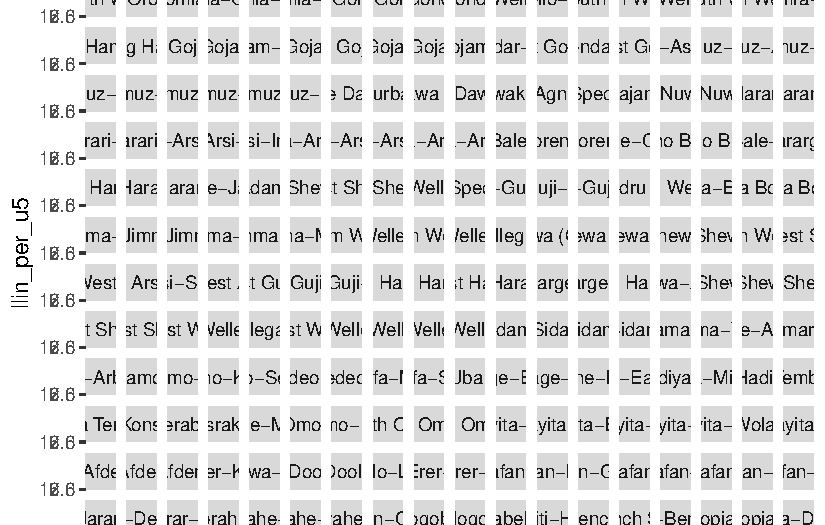
\includegraphics[keepaspectratio]{module_01_files/figure-pdf/unnamed-chunk-6-1.pdf}}

\begin{Shaded}
\begin{Highlighting}[]
 \FunctionTok{ggsave}\NormalTok{(}\AttributeTok{filename =} \StringTok{"plots/llin\_routine.tiff"}\NormalTok{,}
       \AttributeTok{width =} \DecValTok{8}\NormalTok{, }\AttributeTok{height =} \DecValTok{10}\NormalTok{, }\AttributeTok{compression =} \StringTok{"lzw"}\NormalTok{) }
\end{Highlighting}
\end{Shaded}

Unlike mass distributions, routine LLINs are~distributed without
consideration of the size of the population targeted. Rather, they are
handed out during the visits by members of the population. However, we
can have a broad assumption such as that the number of LLINs dispensed
may not exceed the \emph{n} time the population of under-five-year-old
children. Data points flagged in this manner can also be subject to
further scrutiny as part of the~data cleaning process.

\pandocbounded{
\includegraphics[keepaspectratio]{plots/image_01.png}}\hfill

\textbf{Exercise 2:} How many districts in the above example reported
routine LLIN per U5 population values greater than 5 in any year?

\subsection{\texorpdfstring{\textbf{Access to LLIN at the population
level}}{Access to LLIN at the population level}}\label{access-to-llin-at-the-population-level}

Following LLIN distributions LLIN access as a result of the distribution
in the year can be easily estimated. In the next script, we will bring
both mass campaign and routine LLIN distribution data together and
generate estimates of access to LLIN. In calculating access to LLIN at
the~population level,~ will assume one LLIN serves an average of 1.8
individuals in the population.

\begin{Shaded}
\begin{Highlighting}[]
\DocumentationTok{\#\#\# increment to the proportion with access to LLIN}
\NormalTok{llin\_access}\OtherTok{\textless{}{-}}\NormalTok{ mllin\_pop }\SpecialCharTok{|\textgreater{}}
  \FunctionTok{left\_join}\NormalTok{(rllin\_pop,}
            \AttributeTok{by =} \FunctionTok{c}\NormalTok{(}\StringTok{"region"}\NormalTok{, }\StringTok{"zone"}\NormalTok{, }\StringTok{"district"}\NormalTok{, }\StringTok{"year"}\NormalTok{)) }\SpecialCharTok{|\textgreater{}}
  \FunctionTok{mutate}\NormalTok{(}\AttributeTok{total\_llin =}\NormalTok{ llin }\SpecialCharTok{+}\NormalTok{ rllin) }\SpecialCharTok{|\textgreater{}}
  \FunctionTok{mutate}\NormalTok{(}\AttributeTok{llin\_per\_person =}\NormalTok{ total\_llin}\SpecialCharTok{/}\NormalTok{population) }\SpecialCharTok{|\textgreater{}}
  \FunctionTok{mutate}\NormalTok{(}\AttributeTok{inc\_prop\_access =}\NormalTok{ llin\_per\_person}\SpecialCharTok{*}\FloatTok{1.8}\NormalTok{) }\SpecialCharTok{|\textgreater{}}
\NormalTok{  dplyr}\SpecialCharTok{::}\FunctionTok{select}\NormalTok{(region, zone, district, year, total\_llin, llin\_per\_person,}
\NormalTok{                inc\_prop\_access)}

\DocumentationTok{\#\# visualize}
\NormalTok{llin\_access}\SpecialCharTok{|\textgreater{}} 
  \FunctionTok{ggplot}\NormalTok{(}\FunctionTok{aes}\NormalTok{(}\AttributeTok{x=}\NormalTok{year, }\AttributeTok{y =}\NormalTok{ inc\_prop\_access)) }\SpecialCharTok{+}
  \FunctionTok{facet\_wrap}\NormalTok{ (}\SpecialCharTok{\textasciitilde{}}\NormalTok{ district) }\SpecialCharTok{+}
  \FunctionTok{geom\_point}\NormalTok{()}
\end{Highlighting}
\end{Shaded}

\pandocbounded{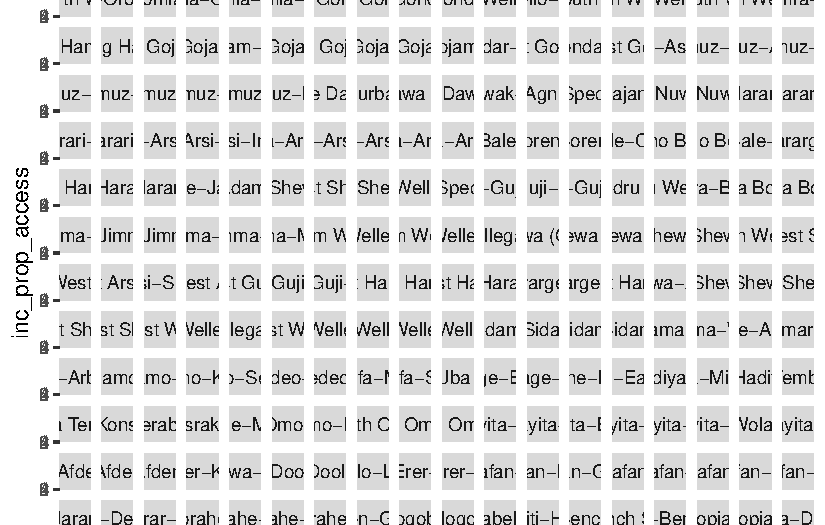
\includegraphics[keepaspectratio]{module_01_files/figure-pdf/unnamed-chunk-7-1.pdf}}

\begin{Shaded}
\begin{Highlighting}[]
\FunctionTok{ggsave}\NormalTok{(}\AttributeTok{filename =} \StringTok{"plots/llin\_access\_increment.tiff"}\NormalTok{,}
       \AttributeTok{width =} \DecValTok{8}\NormalTok{, }\AttributeTok{height =} \DecValTok{10}\NormalTok{, }\AttributeTok{compression =} \StringTok{"lzw"}\NormalTok{)  }
\end{Highlighting}
\end{Shaded}

Since access to LLIN is given in percentages, we can assume a maximum of
1, and districts with values beyond that may be flagged for further
checking of their data. ~

\pandocbounded{
\includegraphics[keepaspectratio]{plots/image_01.png}}\hfill

\textbf{Exercise 3:} How many districts in the above example reported
increment to proportion with access to~ LLIN of greater than 100\%
(\textgreater1.0) ?

\bookmarksetup{startatroot}

\chapter{Demographic and Health
Survey}\label{demographic-and-health-survey}

MACEPA Data Fellowship - Training Materials

\hfill\break

The Demographic and Health Surveys (DHS) program collects data on
health-related indicators at regular intervals (averaging five years) in
many malaria-endemic countries. The DHS collects rare survey data on
malaria indicators, including ITN ownership, ITN usage, indoor residual
spraying coverage, treatment coverage, treatment-seeking rates,
vaccination coverage in the~expanded program on immunization (EPI),
antenatal care coverage, among others.

This module will cover downloading and working with DHS data available
under the \emph{rdhs} package in R.

\bookmarksetup{startatroot}

\chapter{\texorpdfstring{\textbf{Registering with
DHS}}{Registering with DHS}}\label{registering-with-dhs}

All data at the DHS are freely available. However, before you can
download data, you must register as a DHS data user. ~You can register
at this {[}other-links{]}.

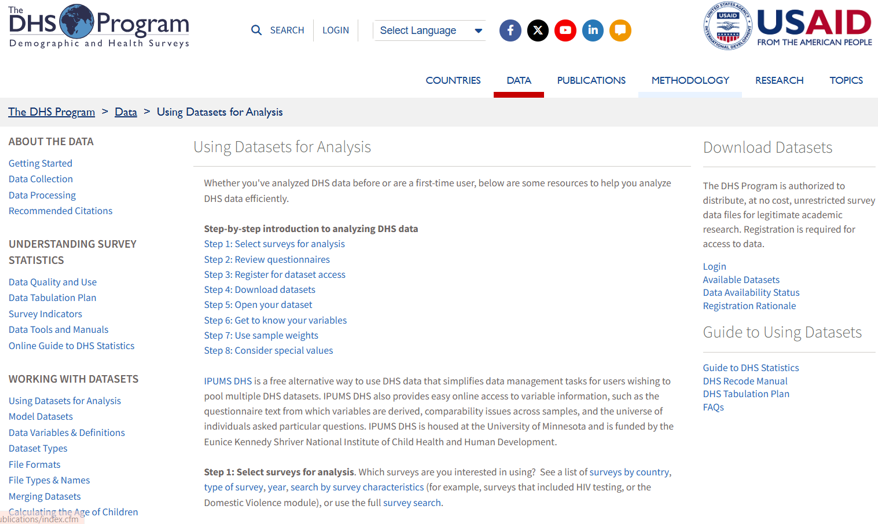
\includegraphics[width=5.41667in,height=\textheight,keepaspectratio]{plots/image_02.png}\hfill

\textbf{Figure 1:} DHS users need to register at this website

In the \emph{Step-by-step introduction to analyzing data} section, you
can select \emph{Step 3:~ Register for dataset access} to get more
information on how to register.

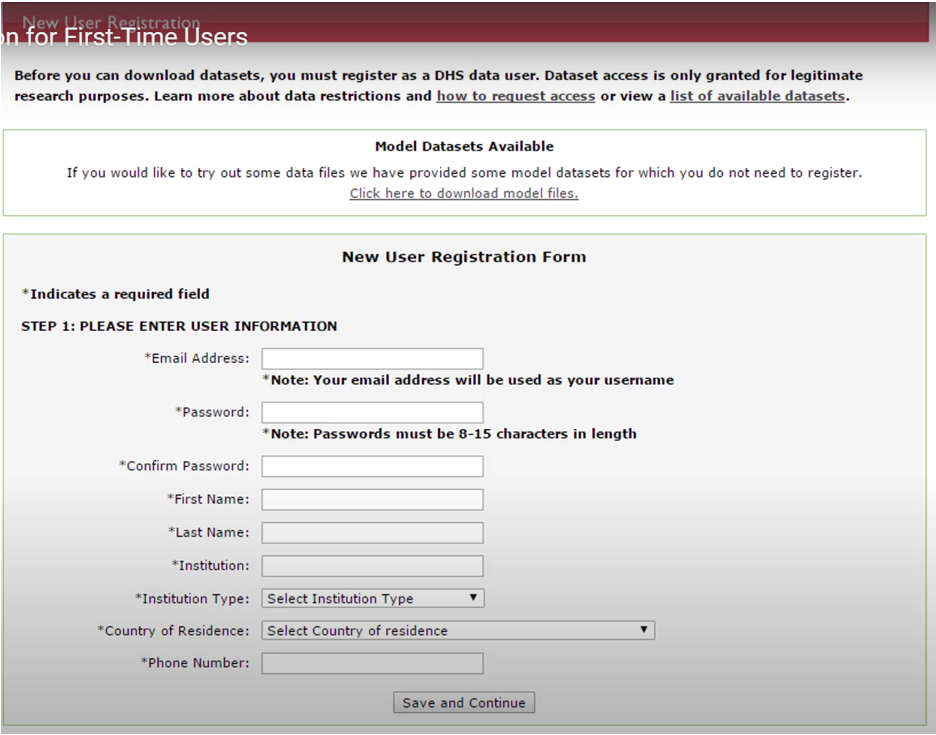
\includegraphics[width=5.20833in,height=\textheight,keepaspectratio]{plots/image_03.png}\hfill

\textbf{Figure 2:} Step 1 of the user registration process

You will need to provide your email and a password which you will use to
access DHS data. Your email address also serves as your username. You
will also need to provide information on the project you will use the
data for. This includes the title, co-researchers, and a description of
the study.~ For our demonstration, we will provide the following
information:

\begin{itemize}
\item
  \textbf{Project Title}: \emph{Malaria control data analysis support}
\item
  \textbf{Co-researcher}: \emph{Name of yout collaborator}
\item
  \textbf{Description of the study}: \emph{The Malaria control data
  analytics support project will work with malaria control programs in
  Africa to strengthen their data-driven decision-making
  process.~Particularly, we aim to answer questions related to alignment
  of program-based data with that from survey data, such as the DHS. We
  will use visualization and statistical tools to answer these
  questions.}
\end{itemize}

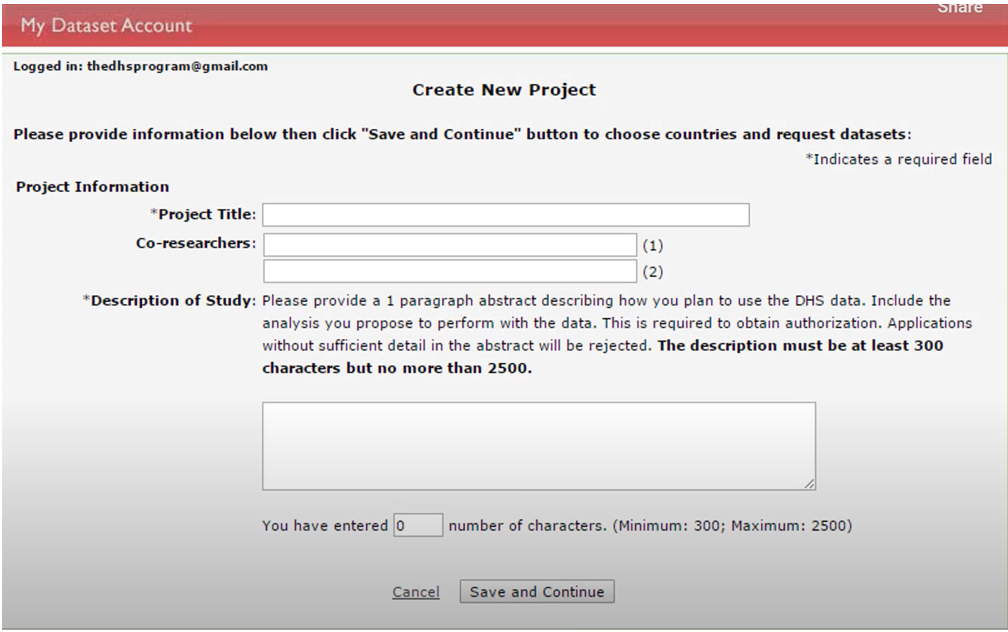
\includegraphics[width=5.41667in,height=\textheight,keepaspectratio]{plots/image_04.png}\hfill

\textbf{Figure 3:} Step 2 of the user registration process

The country/ countries you will download data for may or may not need to
be identified, depending on the project. In this exercise, we will
select the Democratic Republic of Congo (DRC) as the country and
\emph{Sub-Saharan Africa} as the region of interest. You can choose as
many countries as you want, but make sure the list of countries you
select corresponds to the overall objective of the project stated in the
\emph{Description of Study} section.

Once approved, which usually takes 24-48 hours, you will be granted
access to the data

\bookmarksetup{startatroot}

\chapter{\texorpdfstring{\textbf{Exploring the DHS
repository}}{Exploring the DHS repository}}\label{exploring-the-dhs-repository}

Once you have a DHS account, you can access DHS data using the R package
\emph{rdhs}.~ In this section, we will describe the organization of DHS
data in the online DHS archive, accessible through the \emph{rdhs}
package. We will then demonstrate downloading DHS data for DRC.

We begin by installing the \emph{rdhs} package in R and loading the
necessary packages.

\begin{verbatim}
-- Attaching core tidyverse packages ------------------------ tidyverse 2.0.0 --
v dplyr     1.1.4     v readr     2.1.5
v forcats   1.0.0     v stringr   1.5.1
v ggplot2   3.5.2     v tibble    3.3.0
v lubridate 1.9.4     v tidyr     1.3.1
v purrr     1.1.0     
-- Conflicts ------------------------------------------ tidyverse_conflicts() --
x dplyr::filter() masks stats::filter()
x dplyr::lag()    masks stats::lag()
i Use the conflicted package (<http://conflicted.r-lib.org/>) to force all conflicts to become errors

Attaching package: 'janitor'


The following objects are masked from 'package:stats':

    chisq.test, fisher.test


Thank you for using rdhs. If you are using rdhs regularly
or for automated tasks, please register for your own API key by
emailing api@dhsprogram.com. 

More info at <https://api.dhsprogram.com/#/introdevelop.html>
\end{verbatim}

The \emph{rdhs} package has functions that facilitate exploring the DHS
repository.

\section{\texorpdfstring{\textbf{Survey
characteristics}}{Survey characteristics}}\label{survey-characteristics}

To explore what survey types reside in the DHS repository, we can use
the \emph{dhs\_survey\_characteristics()} function. Not all DHS surveys
are related to malaria, and only a few are specific to malaria. You can
find out by filtering those that have ``malaria'' in their names. This
function provides high-level information on the types of data gathered
by the DHS.

\begin{Shaded}
\begin{Highlighting}[]
\CommentTok{\# capture all data on survey characteristics }
\NormalTok{sc}\OtherTok{\textless{}{-}} \FunctionTok{dhs\_survey\_characteristics}\NormalTok{()}
\end{Highlighting}
\end{Shaded}

\begin{verbatim}
Your datasets and API calls will be cached here: 
   -> C:\Users\asiraj\AppData\Local/asiraj/rdhs/Cache
Your datasets will be downloaded using the following config:
\end{verbatim}

\begin{verbatim}
List of 11
 $ email           : NULL
 $ project         : NULL
 $ password        : NULL
 $ cache_path      : chr "C:\\Users\\asiraj\\AppData\\Local/asiraj/rdhs/Cache"
 $ config_path     : chr "C:\\Users\\asiraj\\AppData\\Local/asiraj/rdhs/Cache/rdhs.json"
 $ global          : logi TRUE
 $ verbose_download: logi FALSE
 $ verbose_setup   : logi TRUE
 $ timeout         : int 30
 $ data_frame      : chr "as.data.frame"
 $ project_choice  : NULL
\end{verbatim}

\begin{verbatim}
\end{verbatim}

\begin{Shaded}
\begin{Highlighting}[]
\CommentTok{\# filter those that have \textquotesingle{}malaria\textquotesingle{} in their names}
\NormalTok{mal\_sc}\OtherTok{\textless{}{-}}  \FunctionTok{dhs\_survey\_characteristics}\NormalTok{() }\SpecialCharTok{|\textgreater{}}
\NormalTok{  dplyr}\SpecialCharTok{::}\FunctionTok{filter}\NormalTok{(}\FunctionTok{grepl}\NormalTok{(}\StringTok{"Malaria"}\NormalTok{, SurveyCharacteristicName)) }

\FunctionTok{head}\NormalTok{(mal\_sc)}
\end{Highlighting}
\end{Shaded}

\begin{verbatim}
  SurveyCharacteristicID        SurveyCharacteristicName
1                     96                     Malaria DBS
2                     90              Malaria microscopy
3                    124              Malaria microscopy
4                    119 Malaria microscopy - thin smear
5                     57               Malaria questions
6                     89                     Malaria RDT
\end{verbatim}

\section{Surveys}\label{surveys}

We can go further and explore what country-specific surveys are included
in the repository by using the function dhs\_surveys(). The DHS program
conducts malaria indicator surveys (MISs) in addition to the regular
DHS. MIS is separate from DHS by its \emph{SurveyType} attribute in the
\emph{dhs\_surveys} data set.

\begin{Shaded}
\begin{Highlighting}[]
\CommentTok{\# capture all surveya}
\NormalTok{srv}\OtherTok{\textless{}{-}} \FunctionTok{dhs\_surveys}\NormalTok{ ()}

\CommentTok{\# summarize by survey type}
\FunctionTok{table}\NormalTok{(srv}\SpecialCharTok{$}\NormalTok{SurveyType)}
\end{Highlighting}
\end{Shaded}

\begin{verbatim}

AIS DHS MIS 
 11 313  39 
\end{verbatim}

\begin{Shaded}
\begin{Highlighting}[]
\CommentTok{\# capture MIS surveys by the year of release and country name }
\NormalTok{srv\_mis}\OtherTok{\textless{}{-}} \FunctionTok{dhs\_surveys}\NormalTok{(}\AttributeTok{returnFields =}
                        \FunctionTok{c}\NormalTok{(}\StringTok{"ReleaseDate"}\NormalTok{, }\StringTok{"CountryName"}\NormalTok{,}\StringTok{"SurveyType"}\NormalTok{)) }\SpecialCharTok{|\textgreater{}}
  \FunctionTok{filter}\NormalTok{(SurveyType }\SpecialCharTok{==} \StringTok{"MIS"}\NormalTok{)}

\FunctionTok{head}\NormalTok{(srv\_mis)}
\end{Highlighting}
\end{Shaded}

\begin{verbatim}
  ReleaseDate SurveyType  CountryName
1  2008-02-27        MIS       Angola
2  2012-01-24        MIS       Angola
3  2015-10-16        MIS Burkina Faso
4  2019-07-08        MIS Burkina Faso
5  2013-09-03        MIS      Burundi
6  2023-10-27        MIS     Cameroon
\end{verbatim}

\begin{Shaded}
\begin{Highlighting}[]
\CommentTok{\# display all DHS and MIS surveys released in the year 2018}
\FunctionTok{dhs\_surveys}\NormalTok{(}\AttributeTok{returnFields =}
                        \FunctionTok{c}\NormalTok{(}\StringTok{"ReleaseDate"}\NormalTok{, }\StringTok{"CountryName"}\NormalTok{,}\StringTok{"SurveyType"}\NormalTok{)) }\SpecialCharTok{|\textgreater{}}
  \FunctionTok{filter}\NormalTok{(SurveyType }\SpecialCharTok{\%in\%} \FunctionTok{c}\NormalTok{(}\StringTok{"MIS"}\NormalTok{, }\StringTok{"DHS"}\NormalTok{)) }\SpecialCharTok{|\textgreater{}}
  \FunctionTok{filter}\NormalTok{(}\FunctionTok{year}\NormalTok{(ReleaseDate)}\SpecialCharTok{==}\DecValTok{2018}\NormalTok{)}
\end{Highlighting}
\end{Shaded}

\begin{verbatim}
   ReleaseDate SurveyType CountryName
1   2018-04-05        DHS     Burundi
2   2018-08-21        DHS       Haiti
3   2018-01-11        DHS       India
4   2018-04-25        MIS      Malawi
5   2018-10-03        DHS Philippines
6   2018-09-07        MIS      Rwanda
7   2018-09-28        DHS     Senegal
8   2018-12-14        DHS  Tajikistan
9   2018-10-22        MIS    Tanzania
10  2018-04-10        DHS Timor-Leste
11  2018-08-08        MIS        Togo
12  2018-07-30        DHS      Turkey
13  2018-07-30        DHS      Turkey
14  2018-03-12        DHS      Uganda
\end{verbatim}

\section{Countries}\label{countries}

We can explore which countries have data in the DHS repository by using
the dhs\_countries() function. Notice what country code each country is
assigned. We will use these two-letter country codes to download data in
our examples.

\begin{Shaded}
\begin{Highlighting}[]
\CommentTok{\# capture all countries}
\NormalTok{countries}\OtherTok{\textless{}{-}} \FunctionTok{dhs\_countries}\NormalTok{()}

\CommentTok{\# capture country codes and names}
\NormalTok{country\_ids}\OtherTok{\textless{}{-}} \FunctionTok{dhs\_countries}\NormalTok{(}\AttributeTok{returnFields=}\FunctionTok{c}\NormalTok{(}\StringTok{"DHS\_countryCode"}\NormalTok{, }\StringTok{"CountryName"}\NormalTok{))}

\FunctionTok{head}\NormalTok{(country\_ids)}
\end{Highlighting}
\end{Shaded}

\begin{verbatim}
  DHS_CountryCode CountryName
1              AF Afghanistan
2              AL     Albania
3              AO      Angola
4              AM     Armenia
5              AZ  Azerbaijan
6              BD  Bangladesh
\end{verbatim}

Notice that the country codes for CAR, DRC, Ethiopia, Gambi, Nigeria,
Senegal, and Zambia are ``CF'', ``CD'', ``ET'', ``GM'', ``NG'', ``SN'',
and ``ZM'', respectively.

\section{Indicators}\label{indicators}

DHS (and MIS) include thousands of indicators whose data you can
download These indicators are described in the data dictionary which can
be explored using the \emph{dhs\_indicators()} function.

\begin{Shaded}
\begin{Highlighting}[]
\CommentTok{\#capture the list of indicators}
\NormalTok{ind}\OtherTok{\textless{}{-}} \FunctionTok{dhs\_indicators}\NormalTok{()}
\FunctionTok{names}\NormalTok{(ind)}
\end{Highlighting}
\end{Shaded}

\begin{verbatim}
 [1] "Definition"              "NumberScale"            
 [3] "IndicatorType"           "MeasurementType"        
 [5] "IsQuickStat"             "ShortName"              
 [7] "IndicatorId"             "Level1"                 
 [9] "IndicatorTotalId"        "Level2"                 
[11] "Level3"                  "SDRID"                  
[13] "IndicatorOldId"          "TagIds"                 
[15] "DenominatorWeightedId"   "Label"                  
[17] "IndicatorOrder"          "Denominator"            
[19] "QuickStatOrder"          "IndicatorSpecial1Id"    
[21] "DenominatorUnweightedId" "IndicatorSpecial2Id"    
\end{verbatim}

\begin{Shaded}
\begin{Highlighting}[]
\CommentTok{\#capture the list of indicators by their label and ID}
\NormalTok{indicators }\OtherTok{\textless{}{-}} \FunctionTok{dhs\_indicators}\NormalTok{(}\AttributeTok{returnFields=}\FunctionTok{c}\NormalTok{(}\StringTok{"IndicatorId"}\NormalTok{, }\StringTok{"Label"}\NormalTok{))}

\FunctionTok{head}\NormalTok{(indicators)}
\end{Highlighting}
\end{Shaded}

\begin{verbatim}
    IndicatorId                              Label
1 FE_FRTR_W_A10 Age specific fertility rate: 10-14
2 FE_FRTR_W_A15 Age specific fertility rate: 15-19
3 FE_FRTR_W_A20 Age specific fertility rate: 20-24
4 FE_FRTR_W_A25 Age specific fertility rate: 25-29
5 FE_FRTR_W_A30 Age specific fertility rate: 30-34
6 FE_FRTR_W_A35 Age specific fertility rate: 35-39
\end{verbatim}

\section{Datasets}\label{datasets}

Downloading DHS data involves data retrieval from hundreds of files. The
repository is organized into thousands of datasets, each identified by
its file name. The datasets are stored in different formats, including
SPCC, flat ASCII data, Stata data, etc. The fileType indicates the the
datasets organization including births recode, household members recode,
household recode, provider, verbal autopsy, etc. rdhs uses acronyms to
represent these file types. For instance `PR' is used to represent
person (household member) recode.

\begin{Shaded}
\begin{Highlighting}[]
\CommentTok{\# capture all datasets}
\NormalTok{dset}\OtherTok{\textless{}{-}} \FunctionTok{dhs\_datasets}\NormalTok{()}

\CommentTok{\# capture all datasets by country name, year, file format, and file type. }
\NormalTok{datasets}\OtherTok{\textless{}{-}} \FunctionTok{dhs\_datasets}\NormalTok{(}\AttributeTok{returnFields=}\FunctionTok{c}\NormalTok{(}\StringTok{"SurveyType,"}\NormalTok{, }\StringTok{"CountryName"}\NormalTok{, }\StringTok{"SurveyYear"}\NormalTok{, }\StringTok{"FileFormat"}\NormalTok{, }\StringTok{"FileType"}\NormalTok{))}

\CommentTok{\# capture all datasets related to household member recode}
\NormalTok{person\_datasets}\OtherTok{\textless{}{-}} \FunctionTok{dhs\_datasets}\NormalTok{(}\AttributeTok{fileType =}\StringTok{"PR"}\NormalTok{)}
\end{Highlighting}
\end{Shaded}

\bookmarksetup{startatroot}

\chapter{Downloading DHS data}\label{downloading-dhs-data}

While downloading DHS data involves retrieval of data from corresponding
datasets, in \emph{rdhs} we have the option of downloading data either
specified by the datasets, or a compilation of all data for a specific
country.

At this stage, we need to sign into the DHS repository using the DHS
username and password we have created.~We will use the project we had
registered in the registration section. The process to sign in involves
using the function \emph{set\_rdhs\_config}().

\begin{verbatim}
$email
NULL

$project
NULL

$password
NULL

$cache_path
[1] "C:\\Users\\asiraj\\AppData\\Local/asiraj/rdhs/Cache"

$config_path
[1] "C:\\Users\\asiraj\\AppData\\Local/asiraj/rdhs/Cache/rdhs.json"

$global
[1] TRUE

$verbose_download
[1] FALSE

$verbose_setup
[1] TRUE

$timeout
[1] 30

$data_frame
function (x) 
x
<bytecode: 0x000001a44f149650>
<environment: namespace:base>

$project_choice
NULL

$data_frame_nice
[1] "as.data.frame"

attr(,"class")
[1] "rdhs_config"
\end{verbatim}

\emph{\#this configuration statement enables you to login to your DHS
account}

\emph{set\_rdhs\_config(email = {[}``your email''{]}}

\emph{project = ``Malaria Data Fellowship Program'',}

\emph{config\_path = ``rdhs.json'',}

\emph{global = FALSE)}

To comply with CRAN, this function will also ask you for your permission
to write to files outside your temporary directory, and you must type
out the filename for the config\_path - ``rdhs.json''. The path to your
config is saved between sessions so you only have to set this once. With
your credentials set, all API requests will be cached within the
cache\_path directory provided so that these can be returned when
working remotely or with a poor internet connection. You can also check
your configuration by using the get\_rdhs\_config().

\section{Downloading a specific
dataset}\label{downloading-a-specific-dataset}

Let us assume we want to download RDT prevalence from all surveys
conducted since 2005 in DRC. This can be done by selecting the surveys
conducted since 2025 in DRC, and specifying the file format and file
type.

\begin{itemize}
\item
  Malaria RDT is organized into the survey characteristics named Malaria
  RDT (surveyCharacteristicsId = 89)
\item
  Data on RDT prevalence is located in the dataset organized into
  household members thus will be in household members recode data type
  (PR).
\item
  The file type will be flat ASCII (FL)
\end{itemize}

\begin{Shaded}
\begin{Highlighting}[]
\CommentTok{\# filter the surveys for the DRC (country code CD) and malaria RDT (id=89)}
\CommentTok{\# since 2005}
\NormalTok{this\_survey }\OtherTok{\textless{}{-}} \FunctionTok{dhs\_surveys}\NormalTok{(}
  \AttributeTok{countryIds =} \FunctionTok{c}\NormalTok{(}\StringTok{"CD"}\NormalTok{), }
  \AttributeTok{surveyCharacteristicIds =} \DecValTok{89}\NormalTok{, }
  \AttributeTok{surveyYearStart =} \DecValTok{2005}\NormalTok{)}

\CommentTok{\# zoom into the datasets with data on household member recode}
\NormalTok{this\_dataset }\OtherTok{\textless{}{-}} \FunctionTok{dhs\_datasets}\NormalTok{(}
  \AttributeTok{surveyIds =}\NormalTok{ this\_survey,}
  \AttributeTok{fileFormat =} \StringTok{"FL"}\NormalTok{,}
  \AttributeTok{fileType =} \StringTok{"PR"}\NormalTok{)}

\CommentTok{\# dowload the data from DHS repository}
\CommentTok{\# at this stage the system will verify our login information}

\CommentTok{\# commented out because of a bug at the DHS website}
 \CommentTok{\# downloads \textless{}{-} get\_datasets(this\_dataset$FileName)}
\end{Highlighting}
\end{Shaded}

\section{Downloading all data for a
country}\label{downloading-all-data-for-a-country}

Another approach to downloading DHS data is using the rdhs repository in
R. This repository has archived historical DHS surveys for all countries
, which can access in R. The following script access all DHS data for
DRC conducted since 2005 broken down by provinces.

\begin{Shaded}
\begin{Highlighting}[]
\CommentTok{\# capture all indicators in DHS}
\NormalTok{indicators }\OtherTok{\textless{}{-}} \FunctionTok{dhs\_indicators}\NormalTok{(}\AttributeTok{returnFields=}\FunctionTok{c}\NormalTok{(}\StringTok{"IndicatorId"}\NormalTok{, }\StringTok{"Label"}\NormalTok{))}

\CommentTok{\# capture data on all indicators for the DRC since 2005 }
\CommentTok{\# broken down by subnationally (province level)}
\NormalTok{cd\_all\_dhs}\OtherTok{\textless{}{-}} \FunctionTok{dhs\_data}\NormalTok{(}\AttributeTok{countryIds =} \StringTok{"CD"}\NormalTok{,}
                      \AttributeTok{indicatorIds =}\NormalTok{ indicators}\SpecialCharTok{$}\NormalTok{IndicatorID, }
                      \AttributeTok{surveyYearStart =} \DecValTok{2005}\NormalTok{ ,}
                      \AttributeTok{breakdown =} \StringTok{"subnational"}\NormalTok{)}
\end{Highlighting}
\end{Shaded}

\bookmarksetup{startatroot}

\chapter{Visualization of DHS data}\label{visualization-of-dhs-data}

In the next section, we will exercise visualizing DHS data for
indicators related to vaccination and access to long lasting insecticide
nets (LLINs).

\subsection{LLIN usage}\label{llin-usage}

The DHS indicators for LLIN usage is '\emph{Population who slept under
an insecticide-treated mosquito net (ITN) last night'}. The following
script extracts data specific to this indicator and creates a column
plot showing the LLIN usage proportions at the province level for each
of the survey years.~

\begin{Shaded}
\begin{Highlighting}[]
\DocumentationTok{\#\# indicator/s of interest = LLIN usage (all age)}
\NormalTok{ind}\OtherTok{\textless{}{-}} \StringTok{"Population who slept under an insecticide{-}treated mosquito net (ITN) last night"}

\DocumentationTok{\#\# a column plot for each surveys and provinces}
\NormalTok{cd\_all\_dhs }\SpecialCharTok{|\textgreater{}}
  \FunctionTok{filter}\NormalTok{(Indicator }\SpecialCharTok{\%in\%}\NormalTok{ ind) }\SpecialCharTok{|\textgreater{}}
\NormalTok{janitor}\SpecialCharTok{::}\FunctionTok{clean\_names}\NormalTok{() }\SpecialCharTok{|\textgreater{}}  
  \FunctionTok{rename}\NormalTok{(}\AttributeTok{province=}\NormalTok{characteristic\_label) }\SpecialCharTok{|\textgreater{}}
  \FunctionTok{ggplot}\NormalTok{(}\FunctionTok{aes}\NormalTok{(}\AttributeTok{x=}\NormalTok{province, }\AttributeTok{y =}\NormalTok{ value)) }\SpecialCharTok{+}
  \FunctionTok{facet\_wrap}\NormalTok{(}\SpecialCharTok{\textasciitilde{}}\NormalTok{survey\_year\_label) }\SpecialCharTok{+}
  \FunctionTok{geom\_col}\NormalTok{(}\AttributeTok{position =} \StringTok{"dodge"}\NormalTok{, }\AttributeTok{linewidth =} \FloatTok{1.2}\NormalTok{, }\AttributeTok{fill =} \StringTok{"burlywood2"}\NormalTok{) }\SpecialCharTok{+}
  \FunctionTok{coord\_flip}\NormalTok{() }\SpecialCharTok{+}
  \FunctionTok{labs}\NormalTok{(}\AttributeTok{y=}\StringTok{"Percent"}\NormalTok{, }\AttributeTok{x =} \StringTok{"Province"}\NormalTok{,}
       \AttributeTok{title =}\NormalTok{ ind)}
\end{Highlighting}
\end{Shaded}

\pandocbounded{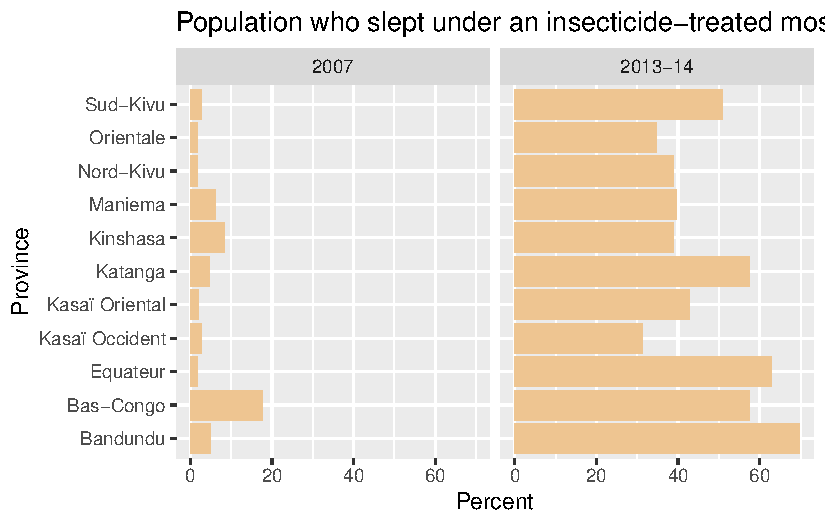
\includegraphics[keepaspectratio]{module_02_files/figure-pdf/unnamed-chunk-10-1.pdf}}

\subsection{LLIN ownership}\label{llin-ownership}

The DHS indicators for LLIN ownership is `\emph{Mean number of
long-lasting insecticide-treated mosquito nets (LLINs) per household}'.
The following script extracts data specific to this indicator and
creates a column plot showing household level LLIN ownership by province
for each of the surveys in DRC.

\begin{Shaded}
\begin{Highlighting}[]
\DocumentationTok{\#\# indicator/s of interest = ITN per household}
\NormalTok{ind}\OtherTok{\textless{}{-}} \StringTok{"Mean number of insecticide{-}treated mosquito nets (ITNs) per household"}
 
\DocumentationTok{\#\# a bar plot for each surveys and provinces}
\NormalTok{cd\_all\_dhs }\SpecialCharTok{|\textgreater{}}
  \FunctionTok{filter}\NormalTok{(Indicator }\SpecialCharTok{\%in\%}\NormalTok{ ind) }\SpecialCharTok{|\textgreater{}}
\NormalTok{  janitor}\SpecialCharTok{::}\FunctionTok{clean\_names}\NormalTok{() }\SpecialCharTok{|\textgreater{}}  
  \FunctionTok{rename}\NormalTok{(}\AttributeTok{province=}\NormalTok{characteristic\_label) }\SpecialCharTok{|\textgreater{}}
  \FunctionTok{mutate}\NormalTok{(}\AttributeTok{year =} \FunctionTok{as.numeric}\NormalTok{(}\FunctionTok{substr}\NormalTok{(survey\_year\_label,}\DecValTok{1}\NormalTok{,}\DecValTok{4}\NormalTok{))) }\SpecialCharTok{|\textgreater{}}
  \FunctionTok{ggplot}\NormalTok{(}\FunctionTok{aes}\NormalTok{(}\AttributeTok{x=} \FunctionTok{as.factor}\NormalTok{(year), }\AttributeTok{y =}\NormalTok{ value, }\AttributeTok{group =}\NormalTok{ province)) }\SpecialCharTok{+}
  \FunctionTok{facet\_wrap}\NormalTok{(}\SpecialCharTok{\textasciitilde{}}\NormalTok{province) }\SpecialCharTok{+}
  \FunctionTok{geom\_col}\NormalTok{(}\AttributeTok{position =} \StringTok{"dodge"}\NormalTok{, }\AttributeTok{size =}\NormalTok{ .}\DecValTok{4}\NormalTok{, }\FunctionTok{aes}\NormalTok{(}\AttributeTok{fill =}\NormalTok{ province)) }\SpecialCharTok{+}
  \FunctionTok{labs}\NormalTok{(}\AttributeTok{y=}\StringTok{"Count"}\NormalTok{, }\AttributeTok{x =} \StringTok{"Year"}\NormalTok{,}
       \AttributeTok{title =}\NormalTok{ ind) }\SpecialCharTok{+}
  \FunctionTok{theme}\NormalTok{(}\AttributeTok{axis.text.x =} \FunctionTok{element\_text}\NormalTok{(}\AttributeTok{angle =} \DecValTok{90}\NormalTok{, }\AttributeTok{vjust =} \FloatTok{0.5}\NormalTok{, }\AttributeTok{hjust=}\DecValTok{1}\NormalTok{),}
        \AttributeTok{legend.position =} \StringTok{"none"}\NormalTok{)}
\end{Highlighting}
\end{Shaded}

\begin{verbatim}
Warning: Using `size` aesthetic for lines was deprecated in ggplot2 3.4.0.
i Please use `linewidth` instead.
\end{verbatim}

\pandocbounded{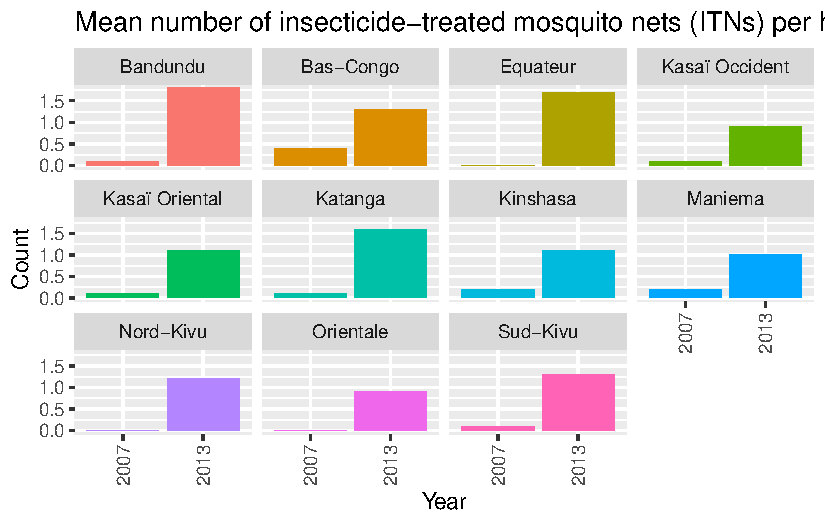
\includegraphics[keepaspectratio]{module_02_files/figure-pdf/unnamed-chunk-11-1.pdf}}

\subsection{RDT prevalence}\label{rdt-prevalence}

The DHS indicators for the prevalence of malaria among children
under-five years old children is `\emph{Malaria prevalence according to
RDT}'. The following script extracts data specific to this indicator and
creates a column plot showing province level RDT based prevalence of
malaria among children.

\begin{Shaded}
\begin{Highlighting}[]
\CommentTok{\#indicator/s of interest = ITN per household}
\NormalTok{ind}\OtherTok{\textless{}{-}} \StringTok{"Malaria prevalence according to RDT"}   

\DocumentationTok{\#\# a column plot for each surveys and provinces }
\NormalTok{cd\_all\_dhs }\SpecialCharTok{|\textgreater{}}
  \FunctionTok{filter}\NormalTok{(Indicator }\SpecialCharTok{\%in\%}\NormalTok{ ind) }\SpecialCharTok{|\textgreater{}}
\NormalTok{    janitor}\SpecialCharTok{::}\FunctionTok{clean\_names}\NormalTok{() }\SpecialCharTok{|\textgreater{}}  
  \FunctionTok{rename}\NormalTok{(}\AttributeTok{province=}\NormalTok{characteristic\_label) }\SpecialCharTok{|\textgreater{}}
  \FunctionTok{ggplot}\NormalTok{(}\FunctionTok{aes}\NormalTok{(}\AttributeTok{x=}\NormalTok{province, }\AttributeTok{y =}\NormalTok{ value)) }\SpecialCharTok{+}
  \FunctionTok{facet\_wrap}\NormalTok{(}\SpecialCharTok{\textasciitilde{}}\NormalTok{survey\_year\_label) }\SpecialCharTok{+}
  \FunctionTok{geom\_col}\NormalTok{(}\AttributeTok{position =} \StringTok{"dodge"}\NormalTok{, }\AttributeTok{size =} \FloatTok{1.2}\NormalTok{, }\AttributeTok{fill =} \StringTok{"indianred3"}\NormalTok{) }\SpecialCharTok{+}
  \FunctionTok{coord\_flip}\NormalTok{() }\SpecialCharTok{+}
  \FunctionTok{labs}\NormalTok{(}\AttributeTok{y=}\StringTok{"Percent"}\NormalTok{, }\AttributeTok{x =} \StringTok{"Province"}\NormalTok{,}
       \AttributeTok{title =}\NormalTok{ ind)}
\end{Highlighting}
\end{Shaded}

\pandocbounded{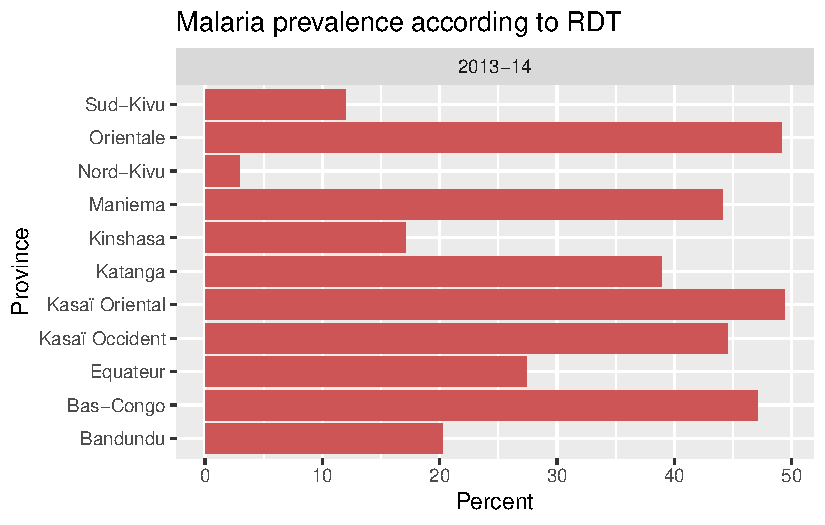
\includegraphics[keepaspectratio]{module_02_files/figure-pdf/unnamed-chunk-12-1.pdf}}

\subsection{Under five mortality}\label{under-five-mortality}

The DHS indicators for the prevalence of malaria among children
under-five years old children is `\emph{Under-five mortality rate}'. The
following script extracts data specific to this indicator and creates a
bar plot showing under five mortality rates by surveys at province
level.

\begin{Shaded}
\begin{Highlighting}[]
\CommentTok{\#indicator/s of interest = U5 mortality }
\NormalTok{ind}\OtherTok{\textless{}{-}} \StringTok{"Under{-}five mortality rate"}     

\DocumentationTok{\#\# a bar plot for each surveys and provinces }
\NormalTok{  cd\_all\_dhs }\SpecialCharTok{|\textgreater{}}   
  \FunctionTok{filter}\NormalTok{(Indicator }\SpecialCharTok{\%in\%}\NormalTok{ ind) }\SpecialCharTok{|\textgreater{}}
\NormalTok{    janitor}\SpecialCharTok{::}\FunctionTok{clean\_names}\NormalTok{() }\SpecialCharTok{|\textgreater{}}  
    \FunctionTok{rename}\NormalTok{(}\AttributeTok{province=}\NormalTok{characteristic\_label) }\SpecialCharTok{|\textgreater{}}
    \FunctionTok{mutate}\NormalTok{(}\AttributeTok{year =} \FunctionTok{as.numeric}\NormalTok{(}\FunctionTok{substr}\NormalTok{(survey\_year\_label,}\DecValTok{1}\NormalTok{,}\DecValTok{4}\NormalTok{))) }\SpecialCharTok{|\textgreater{}}
    \FunctionTok{ggplot}\NormalTok{(}\FunctionTok{aes}\NormalTok{(}\AttributeTok{x=} \FunctionTok{as.factor}\NormalTok{(year), }\AttributeTok{y =}\NormalTok{ value, }\AttributeTok{group =}\NormalTok{ province)) }\SpecialCharTok{+}
    \FunctionTok{facet\_wrap}\NormalTok{(}\SpecialCharTok{\textasciitilde{}}\NormalTok{province) }\SpecialCharTok{+}
    \FunctionTok{geom\_col}\NormalTok{(}\AttributeTok{position =} \StringTok{"dodge"}\NormalTok{, }\AttributeTok{size =}\NormalTok{ .}\DecValTok{4}\NormalTok{, }\AttributeTok{fill =} \StringTok{"indianred3"}\NormalTok{) }\SpecialCharTok{+}
    \FunctionTok{labs}\NormalTok{(}\AttributeTok{y=}\StringTok{"per 1000 live births"}\NormalTok{, }\AttributeTok{x =} \StringTok{"Year"}\NormalTok{,}
       \AttributeTok{title =}\NormalTok{ ind) }\SpecialCharTok{+}
    \FunctionTok{theme}\NormalTok{(}\AttributeTok{axis.text.x =} \FunctionTok{element\_text}\NormalTok{(}\AttributeTok{angle =} \DecValTok{90}\NormalTok{, }\AttributeTok{vjust =} \FloatTok{0.5}\NormalTok{, }\AttributeTok{hjust=}\DecValTok{1}\NormalTok{),}
          \AttributeTok{legend.position =} \StringTok{"none"}\NormalTok{)}
\end{Highlighting}
\end{Shaded}

\pandocbounded{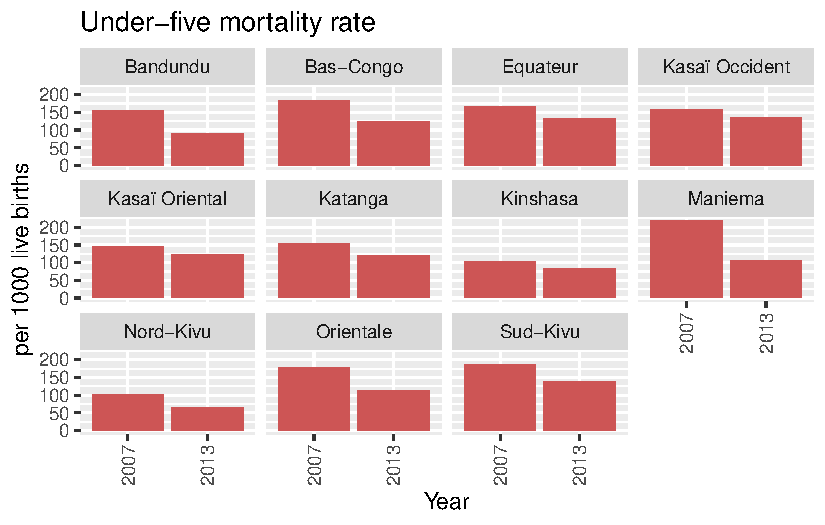
\includegraphics[keepaspectratio]{module_02_files/figure-pdf/unnamed-chunk-13-1.pdf}}

\subsection{DPT3 coverage}\label{dpt3-coverage}

The DHS indicators for the coverage of third dose of DPT based on
vaccination card among children aged 12-23 months old is `DPT 3
vaccination received'. The following script extracts data specific to
this indicator and creates a bar plot showing coverage of DPT-3 s at
province level.

\begin{Shaded}
\begin{Highlighting}[]
\CommentTok{\#indicator/s of interest = DPT 3 coverage }
\NormalTok{ind}\OtherTok{\textless{}{-}} \StringTok{"DPT 3 vaccination received"}       

\DocumentationTok{\#\# a bar plot for each surveys and provinces    }
\NormalTok{cd\_all\_dhs }\SpecialCharTok{|\textgreater{}}      
   \FunctionTok{filter}\NormalTok{(Indicator }\SpecialCharTok{\%in\%}\NormalTok{ ind) }\SpecialCharTok{|\textgreater{}}
\NormalTok{  janitor}\SpecialCharTok{::}\FunctionTok{clean\_names}\NormalTok{() }\SpecialCharTok{|\textgreater{}}  
  \FunctionTok{rename}\NormalTok{(}\AttributeTok{province=}\NormalTok{characteristic\_label) }\SpecialCharTok{|\textgreater{}}
  \FunctionTok{mutate}\NormalTok{(}\AttributeTok{year =} \FunctionTok{as.numeric}\NormalTok{(}\FunctionTok{substr}\NormalTok{(survey\_year\_label,}\DecValTok{1}\NormalTok{,}\DecValTok{4}\NormalTok{))) }\SpecialCharTok{|\textgreater{}}
  \FunctionTok{ggplot}\NormalTok{(}\FunctionTok{aes}\NormalTok{(}\AttributeTok{x=} \FunctionTok{as.factor}\NormalTok{(year), }\AttributeTok{y =}\NormalTok{ value, }\AttributeTok{group =}\NormalTok{ province)) }\SpecialCharTok{+}
  \FunctionTok{facet\_wrap}\NormalTok{(}\SpecialCharTok{\textasciitilde{}}\NormalTok{province) }\SpecialCharTok{+}
  \FunctionTok{geom\_col}\NormalTok{(}\AttributeTok{position =} \StringTok{"dodge"}\NormalTok{, }\AttributeTok{size =}\NormalTok{ .}\DecValTok{4}\NormalTok{, }\AttributeTok{fill =} \StringTok{"honeydew4"}\NormalTok{) }\SpecialCharTok{+}
  \FunctionTok{labs}\NormalTok{(}\AttributeTok{y=}\StringTok{"Percent"}\NormalTok{, }\AttributeTok{x =} \StringTok{"Year"}\NormalTok{,}
       \AttributeTok{title =}\NormalTok{ ind) }\SpecialCharTok{+}
  \FunctionTok{theme}\NormalTok{(}\AttributeTok{axis.text.x =} \FunctionTok{element\_text}\NormalTok{(}\AttributeTok{angle =} \DecValTok{90}\NormalTok{, }\AttributeTok{vjust =} \FloatTok{0.5}\NormalTok{, }\AttributeTok{hjust=}\DecValTok{1}\NormalTok{),}
        \AttributeTok{legend.position =} \StringTok{"none"}\NormalTok{)  }
\end{Highlighting}
\end{Shaded}

\pandocbounded{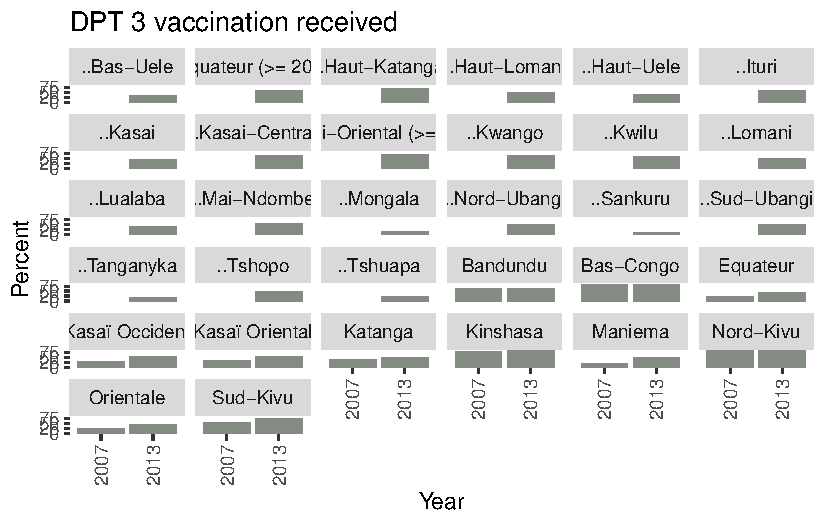
\includegraphics[keepaspectratio]{module_02_files/figure-pdf/unnamed-chunk-14-1.pdf}}




\end{document}
